\documentclass[12pt,a4paper]{article}
\usepackage{amsmath,amscd,amsbsy,amssymb,latexsym,url,bm,amsthm}
\usepackage{epsfig,graphicx,subfigure}
\usepackage{enumitem,balance}
\usepackage{wrapfig}
\usepackage{mathrsfs,euscript}
\usepackage[usenames]{xcolor}
\usepackage{hyperref}
\usepackage{booktabs}
\usepackage[vlined,ruled,linesnumbered]{algorithm2e}
\usepackage{threeparttable}
\hypersetup{colorlinks=true,linkcolor=black}

\newtheorem{theorem}{Theorem}
\newtheorem{lemma}[theorem]{Lemma}
\newtheorem{proposition}[theorem]{Proposition}
\newtheorem{corollary}[theorem]{Corollary}
\newtheorem{exercise}{Exercise}
\newtheorem*{solution}{Solution}
\newtheorem{definition}{Definition}
\theoremstyle{definition}

\renewcommand{\thefootnote}{\fnsymbol{footnote}}

\newcommand{\postscript}[2]
 {\setlength{\epsfxsize}{#2\hsize}
  \centerline{\epsfbox{#1}}}

\renewcommand{\baselinestretch}{1.0}

\setlength{\oddsidemargin}{-0.365in}
\setlength{\evensidemargin}{-0.365in}
\setlength{\topmargin}{-0.3in}
\setlength{\headheight}{0in}
\setlength{\headsep}{0in}
\setlength{\textheight}{10.1in}
\setlength{\textwidth}{7in}
\makeatletter \renewenvironment{proof}[1][Proof] {\par\pushQED{\qed}\normalfont\topsep6\p@\@plus6\p@\relax\trivlist\item[\hskip\labelsep\bfseries#1\@addpunct{.}]\ignorespaces}{\popQED\endtrivlist\@endpefalse} \makeatother
\makeatletter
\renewenvironment{solution}[1][Solution] {\par\pushQED{\qed}\normalfont\topsep6\p@\@plus6\p@\relax\trivlist\item[\hskip\labelsep\bfseries#1\@addpunct{.}]\ignorespaces}{\popQED\endtrivlist\@endpefalse} \makeatother

\providecommand{\limn}{\lim_{n\rightarrow \infty}}
\usepackage{tikz}
\usepackage{pgfplots}
\pgfplotsset{compat=1.14}
\usepgfplotslibrary{colorbrewer}

\begin{document}
\noindent

%========================================================================
\noindent\framebox[\linewidth]{\shortstack[c]{
\Large{\textbf{Lab01-Algorithm Analysis}}\vspace{1mm}\\
CS214-Algorithm and Complexity, Xiaofeng Gao, Spring 2021.}}
\begin{center}
\footnotesize{\color{red}$*$ If there is any problem, please contact TA Haolin Zhou. Also please use English in homework.}

% Please write down your name, student id and email.
\footnotesize{\color{blue}$*$ Name: Zilong Li  \quad Student ID: 518070910095 \quad Email: logcreative-lzl@sjtu.edu.cn}
\end{center}

\begin{enumerate}


\item \textit{Complexity Analysis.} Please analyze the time and space complexity of Alg.~\ref{Alg-quicksort} and Alg.~\ref{Alg-cocktailsort}. \par

\begin{minipage}[t]{0.45\textwidth}
	\begin{algorithm}[H]
		\KwIn{An array $A[1,\cdots,n]$}
		\KwOut{$A[1,\cdots,n]$ sorted nondecreasingly}
		
		\BlankLine
		\caption{QuickSort}\label{Alg-quicksort}
		
		%\If{$n \le 1$}{
		%  \Return\;
		%}
		
		$pivot \leftarrow A[n]$; $i \leftarrow 1$\;
		\For{$j \leftarrow 1$ \KwTo $n-1$}{
			\If{$A[j] < pivot$}{
				swap $A[i]$ and $A[j]$\;
				$i \leftarrow i+1$\;
			}
		}
		
		swap $A[i]$ and $A[n]$\;
		\lIf{$i>1$}{$\operatorname{QuickSort}(A[1,\cdots,i-1])$}
		\lIf{$i<n$}{$\operatorname{QuickSort}(A[i+1,\cdots,n])$}
	\end{algorithm}
\end{minipage}
\hfill
\begin{minipage}[t]{0.45\textwidth}
\begin{algorithm}[H]
\KwIn{An array $A[1,\cdots,n]$}
\KwOut{$A[1,\cdots,n]$ sorted nonincreasingly}
\BlankLine
\caption{CocktailSort}
\label{Alg-cocktailsort}
\BlankLine
	$i\leftarrow 1;$ $j\leftarrow n;$$sorted\leftarrow false$\;
	\While{\textbf{not} sorted}{
		$sorted \leftarrow true$\;
		\For{$k\leftarrow i$ \textbf{to} $j-1$}{
			\If{$A[k] < A[k+1]$}{
				swap $A[k]$ and $A[k+1]$\;
				$sorted\leftarrow false$\;
			}
		}
		$j\leftarrow j-1$\;
		

		\For{$k\leftarrow j$ \textbf{downto} $i+1$}{
			\If{$A[k-1] < A[k]$}{
				swap $A[k-1]$ and $A[k]$\;
				$sorted\leftarrow false$\;
			}
		}
		$i\leftarrow i+1$\;
	}
\end{algorithm}
\end{minipage}

\begin{enumerate}
	 
\item Fill in the blanks and \textbf{explain} your answers. You need to answer when the best case and the worst case happen. 
\begin{table}[!h]

\label{Tab-compare}
	\centering
	\begin{threeparttable}
	\begin{tabular}{c|c| c }
		\toprule[2pt]
		\textbf{Algorithm} & \textbf{Time Complexity}\tnote{1} & \textbf{Space Complexity} \\
		\hline
		\hline
		$QuickSort$ &  &  \\

		$CocktailSort$ &  &   \\
		\bottomrule[2pt]


	\end{tabular}
    \begin{tablenotes}
    	\footnotesize
    	\item[1] The response order can be given in \emph{best}, \emph{average}, and \emph{worst}.
    \end{tablenotes}
	\end{threeparttable}
\end{table}

\item For Alg.~\ref{Alg-quicksort}, how to modify the algorithm to achieve the same expected performance as the \textbf{average} case when the \textbf{worst} case happens?
\end{enumerate} 
\begin{solution}
	\begin{enumerate}
		\item Algorithm \ref{Alg-quicksort} -- QuickSort:
		\begin{description}
			\item[Best Case] 
			\item[Average Case] 
			\item[Worst Case]  
		\end{description}
	\end{enumerate}
\end{solution}

\item \textit{Growth Analysis.} Rank the following functions by order of growth with brief explanations: that is, find an arrangement $g_1, g_2, \ldots , g_{15}$ of the functions $g_1 = \Omega(g_2), g_2 = \Omega(g_3), \ldots, g_{14} = \Omega(g_{15})$.  Partition your list into equivalence classes such that functions $f(n)$ and $g(n)$ are in the same class if and only if $f(n) = \Theta(g(n))$. Use symbols ``$=$'' and ``$\prec$'' to order these functions appropriately. Here $\log n$ stands for $\ln n$.
$$
\begin{array}{ccccc}
	1 \quad & \quad n \quad & \quad \log n \quad & \quad \log (\log n) \quad & \quad n \log n \\
	\log_4 n \quad & \quad 2^n \quad & \quad 4^n \quad & \quad 2^{\log n} \quad & \quad 2^{2^n} \\
	\log (n!) \quad & \quad n! \quad & \quad (2n)! \quad & \quad  n^{1/2} \quad & \quad n^2 \\
\end{array}
$$
\begin{solution}
	Arrangement:
	\begin{equation*}
		2^{2^n},2^{n^2},(2n)!,n!,4^{n},2^n,n^2,n\log n,\log (n!),n,2^{\log n},n^{1/2},\log n,\log \log n,1
	\end{equation*}
	Partition:
	\begin{equation*}
		\begin{aligned}
			1\prec \log\log n\prec \log n\prec n^{1/2}\prec 2^{\log n}\prec n\prec \log (n!)\\= n\log n
			\prec n^2 \prec 2^n \prec 4^{n}\prec n!\prec (2n)!\prec 2^{n^2}\prec 2^{2^n}
		\end{aligned}
	\end{equation*}
	Along the proof, relations \eqref{eq:six} and \eqref{eq:seven} are considered as fundamentals. And Stirling's approximation is used:
	\begin{equation*}
		\limn \frac{n!}{\sqrt{2\pi n}\left(\frac{n}{e}\right)^n} = 1
	\end{equation*}
	L'H\^{o}pital's rule is used: 
	\begin{equation*}
		\limn f(n) = \limn g(n)=+\infty,g^\prime (n)\neq 0,\exists \limn \frac{f^\prime (n)}{g^\prime (n)}\Rightarrow\limn \frac{f(n)}{g(n)} = \limn \frac{f^\prime (n)}{g^\prime (n)}
	\end{equation*}
	The transformation rule of $\omega(\cdot)$ is used:
	\begin{equation*}
		g(n)\neq 0 \Rightarrow \frac{\omega(f(x))}{g(x)} = \omega \left(\frac{f(x)}{g(x)}\right)
	\end{equation*}

	\begin{tikzpicture}
		\begin{semilogyaxis}[solid,
		line width=0.7pt,
		no markers,
		legend pos={outer north east},
		xmin={0},
		xmax={20},
		ymax={1e8},
		height={8.5cm},
		xlabel={$n$},
		axis x line={middle},
		axis y line={left},
		width={14cm},
		grid,samples=21,domain=1:20]
		 \addplot+ [RdYlGn-O,domain=1:7,samples=8] {2^(2^x)};
		 \addplot+ [RdYlGn-N,domain=1:7,samples=8] {2^(x^2)};
		 \addplot+ [RdYlGn-M] {sqrt(2*3.14*2*x)*(2*x/2.71)^(2*x)};
		 \addplot+ [RdYlGn-L] {sqrt(2*3.14*x)*(x/2.71)^x};
		 \addplot+ [RdYlGn-K] {4^x};
		 \addplot+ [RdYlGn-J] {2^x};
		 \addplot+ [RdYlGn-I] {x^2};
		 \addplot+ [RdYlGn-H] {x*ln(x)};
		 \addplot+ [RdYlGn-G] {ln(sqrt(2*3.14*x)*(x/2.71)^x};
		 \addplot+ [RdYlGn-F] {x};
		 \addplot+ [RdYlGn-E] {2^(ln(x))};
		 \addplot+ [RdYlGn-D] {sqrt(x)};
		 \addplot+ [RdYlGn-C] {ln(x)};
		 \addplot+ [RdYlGn-B] {ln(ln(x))};
		%  \addplot+ [black] {1};
		 \legend{$2^{2^n}$,$2^{n^2}$,$(2n)!$,$n!$,$4^{n}$,$2^n$,$n^2$,$n\log n$,$\log (n!)$,$n$,$2^{\log n}$,$n^{1/2}$,$\log n$,$\log \log n$}
		\end{semilogyaxis}
		\end{tikzpicture}

	The proof is as follows:
	\begin{align}
		2^{2^n}=\omega(2^{n^2}) \Leftarrow &&\limn \frac{2^{2^n}}{2^{n^2}} &= \limn 2^{2^n-n^2} = \limn 2^{\omega(n^2)-n^2} = 2^\infty\\
		2^{n^2}=\omega((2n)!) \Leftarrow&& \limn \frac{2^{n^2}}{(2n)!} &= \limn \frac{(2^n)^n}{\sqrt{2\pi(2n)}\left(\frac{n}{e}\right)^n}\nonumber\\
		&& &=\limn \frac{1}{2\sqrt{\pi}}\left(e\frac{2^n}{n}\right)^n\cdot n^{-\frac{1}{2}} \nonumber \\
		&& &= \limn \frac{1}{2\sqrt{\pi}}\left(e\frac{\omega (n^2)}{n}\right)^n\cdot n^{-\frac{1}{2}} \nonumber \\
		&& &=\limn \frac{1}{2\sqrt{\pi}} e^n \omega\left(n^{n-\frac{1}{2}}\right) = \infty \\
		(2n)!=\omega(n!) \Leftarrow&& \limn \frac{(2n)!}{n!} &= \limn\prod_{i=n+1}^{2n} i = \infty \\
		n! = \omega(4^{n}) \Leftarrow&&\limn \frac{n!}{4^n}&=\limn \frac{\sqrt{2\pi n}\left(\frac{n}{e}\right)^n}{4^n}=\infty \\
		4^n = \omega(2^n) \Leftarrow&& \limn \frac{4^n}{2^n} &= \limn 2^n = \infty \\
		2^n = \omega(n^2) \Leftarrow&& \limn \frac{2^n}{n^2}&= \limn \frac{e^{n\log 2}}{n^2} \nonumber\\
		&& &= \limn \frac{1+n\log 2+\frac{(n\log 2)^2}{2}+\frac{(n\log 2)^3}{6}+\omega ((n\log 2)^3)}{n^2} \nonumber\\
		&& &= \limn \left[\alpha + \frac{n \log^3 2}{6} + \omega(n\log^3 2)\right]~(\alpha>0) = \infty\label{eq:six}\\
		n^2 = \omega(n\log n) \Leftarrow&& \limn \frac{n^2}{n\log n}&=\limn \frac{n}{\log n} = \limn \frac{n^\prime}{(\log n)^\prime} = \limn \frac{1}{\frac{1}{n}} = \infty\label{eq:seven}\\
		n\log n = \Theta(\log (n!)) \Leftarrow&& \limn \frac{n\log n}{\log (n!)} &= \limn \frac{n\log n}{\frac{1}{2}\log 2\pi n+n\log n-n} = 1\\
		\log (n!) = \omega(n) \Leftarrow&& \limn \frac{\log (n!)}{n} &= \limn \left(\frac{\pi}{n}+\frac{\log n}{2n} + \log n - 1 \right)=\infty\\
		n=\omega(2^{\log n}) \Leftarrow&& \limn \frac{n}{2^{\log n}}&=\limn \frac{n}{2^{\frac{\log_2 n}{\log_2 e}}} = \limn n^{1-\frac{1}{\log_2 e}}=\limn n^{0.31} = \infty\\
		2^{\log n} = \omega(n^{1/2})\Leftarrow&& \limn \frac{2^{\log n}}{n^{1/2}}&=\limn n^{\frac{1}{\log_2 e}-\frac{1}{2}} = \limn n^{0.19} = \infty \\
		n^{1/2} = \omega(\log n)\Leftarrow&& \limn \frac{n^{1/2}}{\log n}&= \limn \frac{\left(n^{1/2}\right)^\prime}{(\log n)^\prime} = \limn \frac{n^{1/2}}{2} = \infty\\
		\log n = \omega (\log \log n) \Leftarrow&& \limn \frac{\log n}{\log \log n} &= \limn \frac{(\log n)^\prime}{(\log \log n)^\prime} = \limn \frac{1/n}{1/(n\log n)} = \infty \\
		\log\log n = \omega (1) \Leftarrow && \limn \log \log n &= \infty
	\end{align}

\end{solution}


\end{enumerate}

\vspace{20pt}

\textbf{Remark:} You need to include your .pdf and .tex files in your uploaded .rar or .zip file.

%========================================================================
\end{document}
